\documentclass[runningheads]{llncs}

\usepackage[T1]{fontenc}
\usepackage{graphicx}
\usepackage{amsmath,amssymb}
\usepackage{booktabs}
\usepackage{hyperref}
\usepackage{url}
\usepackage{xcolor}
\usepackage{enumitem}
\usepackage{tikz}
\usetikzlibrary{shapes.geometric, arrows.meta, positioning}
\usepackage[left=2.5cm, right=2.5cm, top=2.5cm, bottom=2.5cm]{geometry}
\hypersetup{colorlinks=true, linkcolor=blue, citecolor=blue, urlcolor=blue}

\newcommand{\filepath}[1]{%
  \begingroup\hypersetup{urlcolor=black}\nolinkurl{#1}\endgroup}
\newcommand{\code}[1]{\texttt{#1}}
\newcommand{\ns}[1]{\texttt{news:#1}}

\begin{document}

\title{Automated Knowledge Graph Construction for\\UK Parliamentary and Government Policy Events}
\titlerunning{UK Policy Event KG}
\author{5CCSAKNE Coursework 2}
\authorrunning{5CCSAKNE CW2}
\institute{
    King's College London, London, United Kingdom\\
    \textbf{Repository:}
    \url{https://github.com/ADI-0519/5CCSAKNE-CW2}
}

\maketitle

%------------------------------------------------------------------
\section{Introduction}\label{sec:introduction}
%------------------------------------------------------------------

This project builds an automated knowledge graph (KG) pipeline for UK politics and
policy news (6 March--6 April 2026). The pipeline collects articles from the Guardian
API and NewsAPI, queries the Wikidata SPARQL endpoint for structured UK political
entity data, extracts entities and events from article text, maps both source types to
RDF, enriches the graph through a completion stage, and runs 20 SPARQL competency
queries.

\textbf{Roles:} Abdrakhman Salmenov (domain expert); Aditya Ranjan and Kasim Morsel
(modelling experts); Yingtao Zheng and Immanuel Fradinho Oliveira (data ingestion and
LLM pipeline).

\textbf{Deviations:} NewsAPI developer-tier access returned only 100 results (3 retained
articles), so Wikidata was added as the primary structured source. Legacy
technology-oriented keywords in \filepath{src/config.py} were retained for pipeline
compatibility while the final domain was fixed as UK politics and policy.

\subsection{Technology Stack}

\begin{itemize}[leftmargin=*,nosep]
    \item \textbf{Programming language:} Python.
    \item \textbf{Knowledge graph stack:} RDF, Turtle, SPARQL, and \code{rdflib}.
    \item \textbf{Sources:} Guardian API, UK Parliament written-statements API,
    GOV.UK Search API, and optional Wikidata SPARQL enrichment.
    \item \textbf{LLM integration:} OpenAI structured extraction support with
    schema validation and local caching.
    \item \textbf{Testing:} \code{pytest} tests for ontology construction,
    normalisation, RDF generation, completion, and query execution.
\end{itemize}

%------------------------------------------------------------------
\section{Data Sources}\label{sec:data_sources}
%------------------------------------------------------------------

The coursework requires at least one textual and one structured source.

\begin{itemize}[leftmargin=*,nosep]
    \item \textbf{Guardian API (textual):} full \code{bodyText} content for NLP
    extraction. 253 articles retained. Implemented in \filepath{src/data\_collection.py}.
    \item \textbf{Wikidata SPARQL endpoint (structured):} typed entity records for UK
    politicians (1730), political parties (968), and government bodies (490),
    mapped directly to RDF without NLP. Implemented in
    \filepath{src/wikidata\_collection.py}.
    \item \textbf{UK Parliament + GOV.UK APIs:} 20 parliamentary and 459 government
    records used as official source records.
    \item \textbf{NewsAPI (supplementary):} 3 articles retained after scope filtering.
\end{itemize}

The Guardian was chosen for its full body text enabling genuine extraction. Wikidata
was chosen for its public SPARQL endpoint and typed political actor data requiring no
API key. Raw snapshots are saved under \filepath{data/raw/}, allowing cached reruns.
Source selection prompts are logged in \filepath{prompts/prompts.txt}.

%------------------------------------------------------------------
\section{Ontology Design}\label{sec:ontology_design}
%------------------------------------------------------------------

The ontology is built programmatically in \filepath{src/build\_ontology.py} and
serialised to \filepath{ontology/news\_ontology.ttl}. It extends \textbf{Schema.org}
(articles, people, organisations, metadata) and the \textbf{BBC Core Concepts Ontology}
(events, places) under the \code{news:} namespace.

\begin{table}[t]
\centering
\caption{Core ontology extensions.}\label{tab:ontology}
\setlength{\tabcolsep}{5pt}
\begin{tabular}{@{}p{2.7cm}p{9.3cm}@{}}
\toprule
\textbf{Layer} & \textbf{Implemented terms} \\
\midrule
Events & \ns{PolicyEvent}, \ns{ParliamentaryEvent}, \ns{GovernmentPolicyEvent}, \ns{ParliamentaryDebate}, \ns{MinisterialStatement} \\
Actors and institutions & \ns{PoliticalActor}, \ns{PoliticalParty}, \ns{OfficialBody}, \ns{GovernmentBody}, \ns{GovernmentDepartment}, \ns{ParliamentaryBody} \\
Topics and places & \ns{PolicyTopic}, \ns{Location} \\
Reporting and provenance & \ns{NewsArticle}, \ns{NewsOrganisation}, \ns{Journalist}, \ns{SourceRecord}, \ns{OfficialSourceRecord}, \ns{ParliamentSourceRecord}, \ns{GovernmentSourceRecord} \\
\bottomrule
\end{tabular}
\end{table}

\ns{PolicyEvent} extends \code{core:Event}; \ns{Location} extends \code{core:Place};
\ns{NewsArticle} extends \code{schema:NewsArticle}; \ns{OfficialBody} extends
\code{schema:Organization}. Properties such as \ns{concernsPolicyTopic},
\ns{occursInLocation}, \ns{publishedBy}, and \ns{hasAuthor} are aligned with
Schema.org or BBC Core Concepts, satisfying the subclass and subproperty requirements.

%------------------------------------------------------------------
\section{Mappings}\label{sec:mappings}
%------------------------------------------------------------------

The pipeline implements two separate mapping paths.

\textbf{Textual path (Guardian + NewsAPI):} \filepath{src/data\_extraction.py}
combines heuristic and optional OpenAI-assisted extraction. The heuristic layer
identifies people, organisations, and locations via controlled lists and regex;
topics via weighted keyword groups; article subtype; and event candidates. The OpenAI
layer uses strict JSON-schema outputs, validated before use and cached under
\filepath{data/cache/openai/}. Extracted records are converted to RDF by \filepath{src/json\_to\_rdf.py}.

\textbf{Structured path (Wikidata):} \filepath{src/wikidata\_to\_rdf.py} converts
SPARQL results to RDF by direct field-to-property mapping with no NLP.

Official Parliament and GOV.UK records are typed as source records and linked to events
through \ns{representedInOfficialSource}. Figure~\ref{fig:pipeline} shows the
end-to-end pipeline.

\begin{figure}[t]
\centering
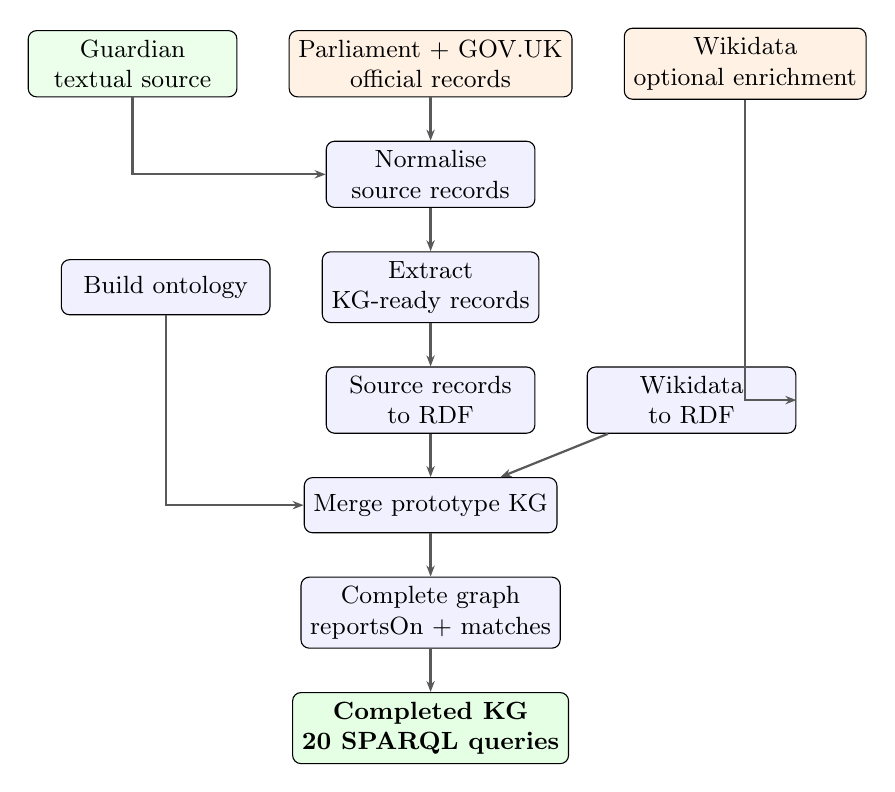
\begin{tikzpicture}[
  node distance=0.55cm and 0.65cm,
  block/.style={draw, rounded corners=3pt, fill=blue!6, minimum height=0.70cm, minimum width=2.65cm, font=\small, align=center},
  output/.style={draw, rounded corners=3pt, fill=green!10, minimum height=0.75cm, minimum width=2.9cm, font=\small\bfseries, align=center},
  arrow/.style={-{Stealth[length=4pt]}, thick, color=black!65}
]
  \node[block, fill=green!8] (guardian) {Guardian\\textual source};
  \node[block, right=of guardian, fill=orange!10] (official) {Parliament + GOV.UK\\official records};
  \node[block, right=of official, fill=orange!10] (wiki) {Wikidata\\optional enrichment};
  \node[block, below=of official] (norm) {Normalise\\source records};
  \node[block, below=of norm] (extract) {Extract\\KG-ready records};
  \node[block, left=of extract] (onto) {Build ontology};
  \node[block, below=of extract] (rdf) {Source records\\to RDF};
  \node[block, right=of rdf] (wikirdf) {Wikidata\\to RDF};
  \node[block, below=of rdf] (merge) {Merge prototype KG};
  \node[block, below=of merge] (complete) {Complete graph\\reportsOn + matches};
  \node[output, below=of complete] (query) {Completed KG\\20 SPARQL queries};

  \draw[arrow] (guardian) |- (norm);
  \draw[arrow] (official) -- (norm);
  \draw[arrow] (wiki) |- (wikirdf);
  \draw[arrow] (norm) -- (extract);
  \draw[arrow] (extract) -- (rdf);
  \draw[arrow] (onto) |- (merge);
  \draw[arrow] (rdf) -- (merge);
  \draw[arrow] (wikirdf) -- (merge);
  \draw[arrow] (merge) -- (complete);
  \draw[arrow] (complete) -- (query);
\end{tikzpicture}
\caption{End-to-end pipeline used in the current codebase.}
\label{fig:pipeline}
\end{figure}

%------------------------------------------------------------------
\section{Competency Questions}\label{sec:cq}
%------------------------------------------------------------------

The project defines 20 competency questions in
\filepath{docs/competency_questions.md}. Ten were manually authored from the
domain requirements and ten were generated with LLM assistance before manual
revision. They are implemented as SPARQL queries in
\filepath{queries/news_competency_queries.rq}.

The questions deliberately exercise non-trivial ontology paths, including:

\begin{itemize}[leftmargin=*,nosep]
    \item event-to-topic retrieval;
    \item ministerial-statement-to-department links;
    \item actor, party, and topic aggregation;
    \item official-source representation and source-system provenance;
    \item publisher and journalist paths through articles to events;
    \item diagnostic missing-link queries for completion analysis.
\end{itemize}

%------------------------------------------------------------------
\section{KG Completion}\label{sec:completion}
%------------------------------------------------------------------

The completion stage (\filepath{src/complete\_kg.py}) identified missing source-integration
links in the prototype graph and enriched it with ontology-aligned triples. Five gap
types were targeted: missing \ns{reportsOn} links from articles to events, missing
\ns{matchedToSourceRecord} links between events and official records, missing actor
links, missing department links, and incomplete topic assignments. The stage added 504
triples: 266 inverse \ns{reportsOn} links and 238 \ns{matchedToSourceRecord} links.
A RAG step retrieves article headlines and source titles via SPARQL, verbalises the
context, and prompts OpenAI with a closed vocabulary to propose actor, department, and
topic values, which are validated before merging.

%------------------------------------------------------------------
\section{Prompts}\label{sec:prompts}
%------------------------------------------------------------------

Eight prompts were versioned and logged in \filepath{prompts/prompts.txt}:
(1)~pipeline planning; (2)~CQ augmentation; (3)~ontology review;
(4)~source-to-ontology mapping; (5)~completion gap analysis;
(6)~evaluation methodology; (7)~runtime entity and event extraction;
(8)~runtime KG completion.
Prompts 1--6 were used during design and revised manually. Prompts 7--8 execute at
runtime with strict JSON-schema validation before outputs enter the graph.

%------------------------------------------------------------------
\section{Evaluation}\label{sec:evaluation}
%------------------------------------------------------------------

The latest validated run is \code{20260420T202251Z}. All 20 competency queries returned
at least one row.

\begin{table}[t]
\centering
\caption{Summary statistics for the evaluated run.}
\label{tab:stats}
\begin{tabular}{@{}lr@{}}
\toprule
\textbf{Measure} & \textbf{Value} \\
\midrule
Guardian records & 253 \\
Parliament / GOV.UK records & 20 / 459 \\
Wikidata politicians / parties / gov.\ bodies & 1730 / 968 / 490 \\
Ontology graph & 188 triples \\
Prototype KG & 39545 triples \\
Completed KG & 40049 triples \\
Queries returning at least one row & 20 / 20 \\
\bottomrule
\end{tabular}
\end{table}

\begin{table}[t]
\centering
\caption{Competency-query row counts for the completed KG.}
\label{tab:queries}
\begin{tabular}{@{}lrrrrrrrrrr@{}}
\toprule
CQ & 01 & 02 & 03 & 04 & 05 & 06 & 07 & 08 & 09 & 10 \\
\midrule
Rows & 15 & 25 & 11 & 233 & 3 & 4 & 8 & 4 & 193 & 12 \\
\bottomrule
\end{tabular}

\vspace{0.5em}

\begin{tabular}{@{}lrrrrrrrrrr@{}}
\toprule
CQ & 11 & 12 & 13 & 14 & 15 & 16 & 17 & 18 & 19 & 20 \\
\midrule
Rows & 81 & 11 & 48 & 12 & 7 & 8 & 11 & 11 & 1 & 8 \\
\bottomrule
\end{tabular}
\end{table}

\textbf{Quality:} The KG is most reliable for article metadata, publisher and author
information, topic assignment, and source traceability. Weaker areas: person and
organisation extraction over-generates via regex; event labels remain generic; the
corpus is Guardian-dominated.

\textbf{KG vs.\ direct LLM:} KG-based answers are reproducible, auditable, and grounded
in structured triples. Direct LLM prompting is more fluent but non-deterministic and
non-traceable.

%------------------------------------------------------------------
\section{Testing and Reproducibility}\label{sec:testing}
%------------------------------------------------------------------

Automated \code{pytest} tests under \filepath{tests/} cover ontology construction,
RDF generation, completion, and query execution. Reproducibility is supported through
saved raw snapshots, timestamped processed JSON outputs, and cached source runs
(\code{--from-cache}).

%------------------------------------------------------------------
\section{Conclusion}\label{sec:conclusion}
%------------------------------------------------------------------

The repository delivers a working automated KG pipeline for UK parliamentary and
government policy events. The system is reproducible, ontology-aligned, and queryable,
with all 20 competency questions answered. Remaining work includes entity resolution,
event canonicalisation, and richer provenance for completion links.

\newpage
\begin{thebibliography}{9}

\bibitem{schema}
Schema.org: \url{https://schema.org/}

\bibitem{bbc}
BBC Core Concepts Ontology: \url{http://www.bbc.co.uk/ontologies/coreconcepts/}

\bibitem{rdf}
W3C: RDF 1.1 Concepts and Abstract Syntax. \url{https://www.w3.org/TR/rdf11-concepts/}

\bibitem{sparql}
W3C: SPARQL 1.1 Query Language. \url{https://www.w3.org/TR/sparql11-query/}

\bibitem{guardian}
The Guardian Open Platform: \url{https://open-platform.theguardian.com/}

\bibitem{parliament}
UK Parliament Questions and Statements API: \url{https://questions-statements-api.parliament.uk/}

\bibitem{govuk}
GOV.UK Search API: \url{https://www.gov.uk/api/search.json}

\bibitem{wikidata}
Wikidata Query Service: \url{https://query.wikidata.org/}

\bibitem{openai}
OpenAI API documentation: \url{https://platform.openai.com/docs}

\end{thebibliography}

\end{document}
